\chapter{Resultados}\label{ch:resultados}


\section{Resultados relativos al objetivo 1}\label{sec:resultados-relativos-al-objetivo-1}

Los resultados de este objetivo corresponden al desarrollo
de un \textbf{sistema de vinculación de componentes} para el
entorno de desarrollo integrado \textit{JAMS},
permitiendo a otros desarrolladores aportar nuevas funcionalidades
a la aplicación de manera sencilla.

Se considera que \textbf{se ha superado con creces} \note{Óscar: ya hemos hablado de esto en el otro TFG. Pues lo mismo} este objetivo.
El sistema de vinculación de componentes desarrollado permite
instalar y desinstalar componentes sin que el usuario tenga
que reiniciar la aplicación.
Además, mediante el sistema de dependencias débiles y fuertes,
los componentes pueden \textbf{interactuar entre s\delODR{i}\newODR{í}}, añadiendo
más flexibilidad a los desarrolladores.

\begin{figure}[h]
    \centering
    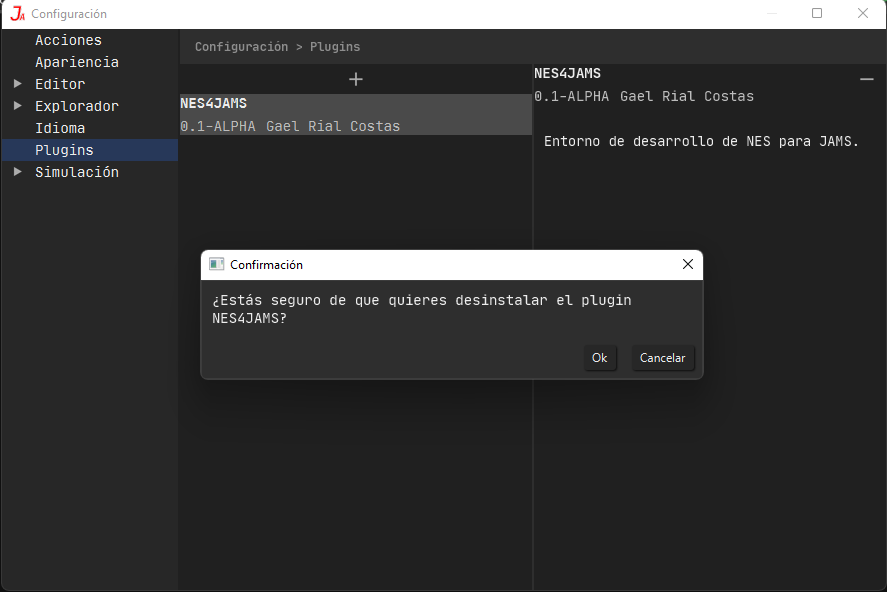
\includegraphics[width=0.8\textwidth]{images/results/jams-uninstall}
    \caption{Desinstalación de un componente}
    \label{fig:jams-uninstall}
\end{figure}

El hecho de que \textit{JAMS} esté desarrollado en \textit{Java}
ha permitido simplificar mucho el desarrollo de este sistema
de vinculación.
Gracias a las librerías presentes en el \textit{JDK} para cargar
código externo, \textit{JAMS} puede gozar de un sistema de componentes
muy sólido.

El sistema de \textbf{proveedores} desarrollado para los elementos
proporcionados por los componentes también ha resultado ser un éxito.
Este sistema permite que ninguna referencia a ninguna clase de un
componente quede referenciada en \textit{JAMS} cuando dicho componente
se desinstala.
Sin el sistema de proveedores, la desinstalación sería imposible debido
a los errores que la desinstalación podría causar.


\section{Resultados relativos al objetivo 2}\label{sec:resultados-relativos-al-objetivo-2}

Los resultados de este objetivo corresponden al desarrollo y mejora de
\textbf{diversas tecnologías} para permitir a los componentes modificar
todos los aspectos de \textit{JAMS} de una manera rápida y sencilla.

Este objetivo se considera superado de manera satisfactoria\note{Óscar:Idem}.
La tecnología desarrollada más usada por los componentes
y por el propio \textit{JAMS} ha sido el sistema de \textbf{gestores},
el cual ha permitido gestionar los elementos de la aplicación
de una manera rápida y sencilla, haciendo que los componentes
puedan añadir nuevos elementos de manera transparente.
Este sistema es complementado por los \textbf{eventos},
los cuales permiten recibir información sobre los sucesos que
acontecen en el entorno de desarrollo.
Con ambos sistemas combinados, tanto \textit{JAMS} como los componentes
pueden refrescar su información fácilmente cuando algún elemento
de un gestor es añadido o eliminado.

\begin{figure}[h]
    \centering
    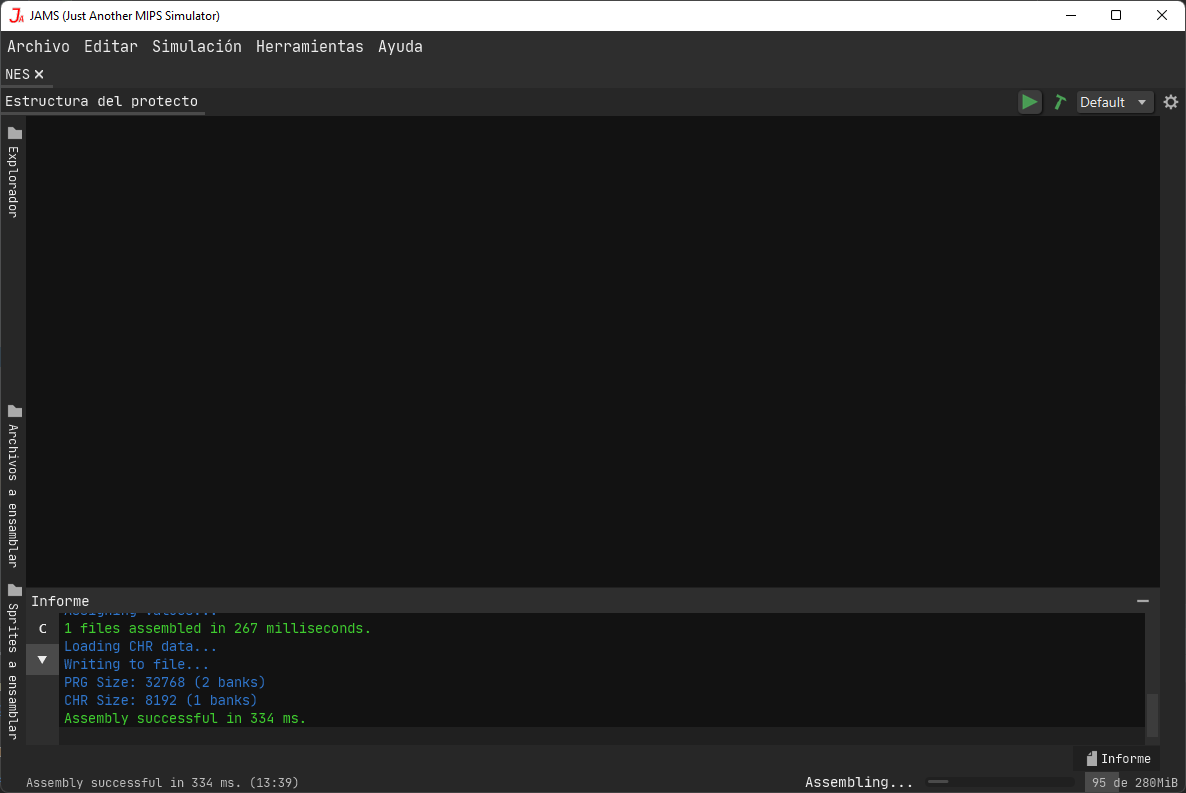
\includegraphics[width=0.8\textwidth]{images/results/jams-tasks}
    \caption{Barra de tareas informando sobre el ensamblaje}
    \label{fig:jams-tasks}
\end{figure}

Otra tecnología muy utilizada han sido las \textbf{tareas},
las cuales permiten ejecutar código asíncrono de una manera muy
sencilla.
Añadir un ejecutor de tareas en cada proyecto ha sido un
absoluto \textbf{acierto}\note{Óscar: ibidem}: gracias a tener todas las tareas
de un proyecto agrupadas en un ejecutor, se ha podido añadir
un elemento en la barra inferior de la aplicación que muestra
el proceso de todas las tareas del proyecto actual,
tal como se observa en la figura \ref{fig:jams-tasks}.

\section{Resultados relativos al objetivo 3}\label{sec:resultados-relativos-al-objetivo-3}

Los resultados de este objetivo corresponden al desarrollo
de un componente que añada a \textit{JAMS} un \textbf{entorno de
desarrollo integrado} para la creación de videojuegos de la
consola \textit{NES}, incorporando un editor de código
y de gráficos, un ensamblador y un simulador.

Este objetivo también se considera superado de manera satisfactoria.
El nuevo componente permite desarrollar videojuegos de
la \textit{NES} usando un editor de código muy similar al encontrado
en el entorno de desarrollo para \textit{MIPS32}, incorporando
herramientas como el \textbf{autocompletador} o el \textbf{inspector de código},
agilizando el desarrollo de los videojuegos.
El componente también presenta un editor de gráficos, el cual permite
editar los patrones presentes en las tablas del juego.

\begin{figure}[h]
    \centering
    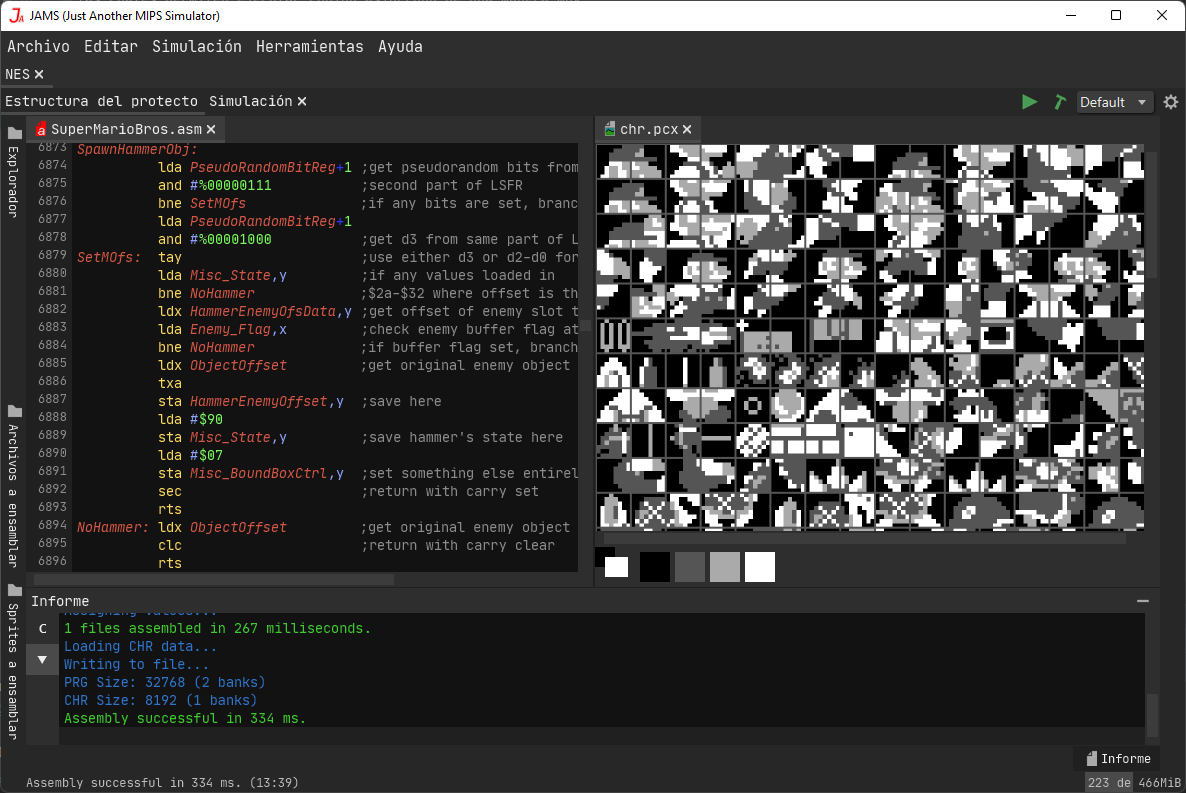
\includegraphics[width=0.8\textwidth]{images/results/nes-editor}
    \caption{Editor de código y de gráficos}
    \label{fig:nes-result-editor}
\end{figure}

El ensamblador, inspirado por el ensamblador presente
en \textit{JAMS} para la arquitectura \textit{MIPS32},
incorpora varias características avanzadas no encontradas
en ensambladores más sencillos, como lo son las referencias
relativas o las macros anidadas.
Este ensamblador escribe el resultado en un archivo \textit{iNES},
lo que permite al desarrollador distribuir su videojuego de manera
sencilla.

Por último, \textit{NES4JAMS} incorpora un simulador de la arquitectura
de la consola \textit{NES} que permite ejecutar la mayoría de los
videojuegos comerciales.
Este simulador permite visualizar el estado del videojuego desde varios
puntos de vista gracias a las herramientas incluidas.
La herramienta más característica del simulador es la herramienta
\textit{PPU}, la cual permite visualizar de manera muy visual el estado
de la unidad de procesamiento de imágenes,
como se observa en la figura \ref{fig:nes-result-simulator}.

\begin{figure}[h]
    \centering
    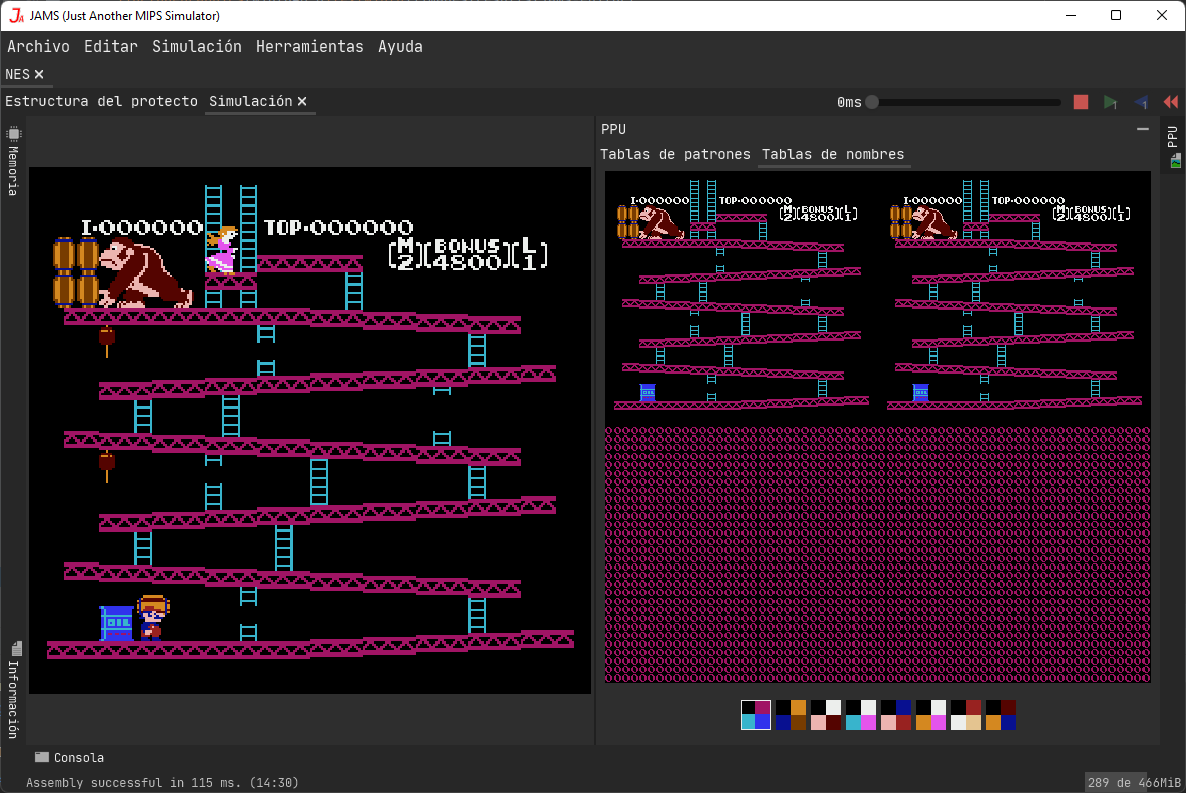
\includegraphics[width=0.8\textwidth]{images/results/nes-simulator}
    \caption{Simulador con la herramienta \textit{PPU}}
    \label{fig:nes-result-simulator}
\end{figure}

Todos estos elementos conforman un entorno de desarrollo
\textbf{sólido} para la creación de nuevos videojuegos
para la \textit{NES}.

Por último, cabe destacar que la elección del lenguaje
de programación \textit{Kotlin} para el desarrollo de
este componente ha sido una \textbf{gran elección}.
Su diseño más conciso, combinado con nuevas características
como el soporte para números sin signos, ha permitido
acelerar el ritmo de desarrollo del componente.
La capacidad de \textit{Kotlin} de poder ejecutar sus
programas en la \textit{JVM} permite que se puedan
crear componentes para \textit{JAMS} en este lenguaje
de programación de manera \textbf{transparente}, sin
tener el desarrollador que ejecutar ningún paso intermedio.
